\section*{Assignment 08: Metrics and Learning}
\addcontentsline{toc}{section}{Assignment 08: Metrics and Learning}

This section focuses on the metrics that would keep SkillSync effective each week rather than on a theoretical appendix.

\subsection*{KPIs that make sense}
\begin{itemize}
    \item \textbf{Matching rate}: Share of suggested matches that land; if it drops we tweak the algorithm or onboarding questions and slice by cohort.
    \item \textbf{Repeat usage rate}: Share of users who return within 30 days; a dip triggers a review of retention features or community rituals.
    \item \textbf{Net Promoter Score}: Signals whether people would recommend us. Drops usually flag fairness issues or bugs, so we pair them with quick interviews.
    \item \textbf{Time-to-first-value}: Minutes to the first meaningful interaction. When it drags, we strip friction or add guided missions.
    \item \textbf{Revenue per active match}: Keeps monetisation tied to behaviour while we monitor variance so a few power users do not prop up the number.
    \item \textbf{Equity of participation}: Share of projects from resource-light partners so we track inclusion goals from Assignment~07.
    \item \textbf{Partner retention}: Share of organisations posting again within 60 days. It keeps the organisation side visible in planning debates.
\end{itemize}

\subsection*{Data infrastructure and feedback loop}
I keep the data stack simple on paper. Events would land in a cloud warehouse (BigQuery or Snowflake) because both scale affordably and support granular access controls. Data would stream via Segment or RudderStack so the app stays decoupled, dbt shapes clean tables for analysis, and dashboards live in Looker Studio or Metabase so anyone can explore without SQL while respecting permissions.

The feedback loop runs on three rhythms in the plan, mirroring the instrumentation drills from Lecture~5 on metrics and experimentation \citep{Lecture05}:
\begin{itemize}
    \item \textbf{Weekly reviews}: Product, data, and support meet every Tuesday, walk the KPI dashboard, and check fresh cohorts so onboarding issues surface fast.
    \item \textbf{Monthly cohort analyses}: Segment by acquisition channel and first-match timestamp to see which cohorts stick and pay; the report feeds marketing spend and the roadmap.
    \item \textbf{Quarterly learning readouts}: Summarise experiments, share surprises, and reset hypotheses so the informal student vibe still produces structured knowledge.
\end{itemize}

\subsection*{How metrics guide change}
Imagine matching rate drops from 62\% to 48\% over three weeks. A weekly review would show new users from a partner campaign lagging and cohort analysis would reveal time-to-first-value above 48 hours. I would run an onboarding A/B test, add a preference step, tighten algorithm weights, and ship the winner two sprints later. The next monthly check in this scenario shows matching back above 60\%, repeat usage up eight points, revenue per active match nudging upward, and equity of participation intact, turning KPIs into a compass instead of decoration.

Figure~\ref{fig:feedback-screen} shows the feedback interface powering these metrics: after each project both sides rate collaboration quality, delivery against scope, and communication cadence while qualitative notes surface for moderation and scores feed the matching algorithm. ``Impact badges'' reinforce good behaviour while the layout keeps the UX light.

\begin{figure}[H]
  \centering
  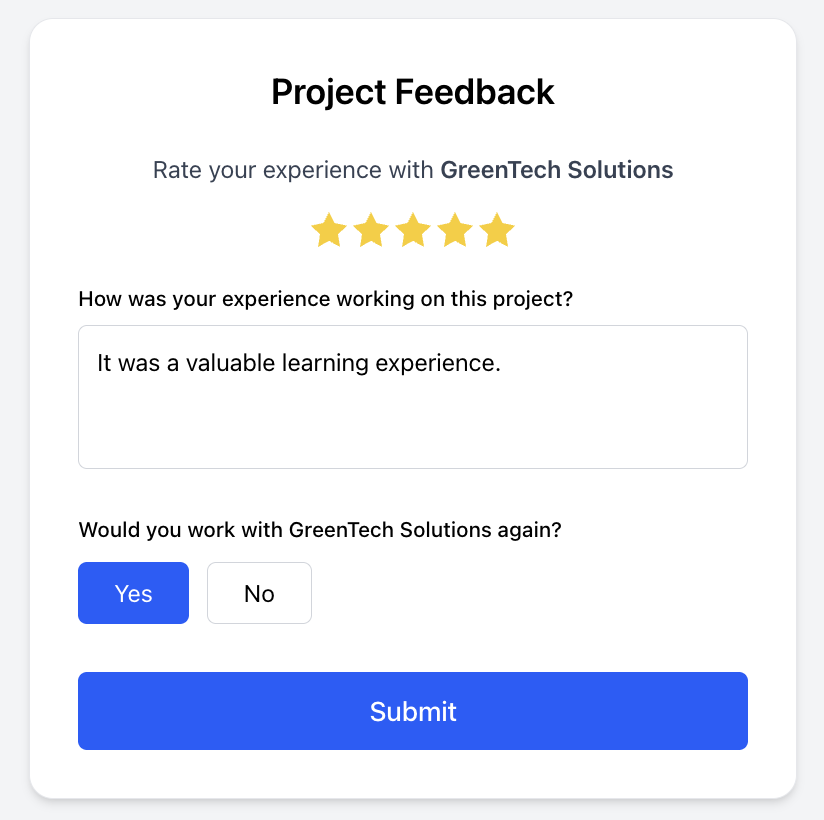
\includegraphics[width=0.8\linewidth]{figures/Student-Project-Feedback.png}
  \caption{Feedback screen mock-up balancing qualitative notes and structured scores.}
  \label{fig:feedback-screen}
\end{figure}

I keep the analytics stack geared toward reproducibility. Dashboards would carry ``definition'' tooltips that link to the dbt logic, SQL lives in version control, and a metrics catalogue keeps newcomers oriented. Quarterly KPI snapshots would preserve history even as definitions evolve, turning metrics into institutional memory in the spirit of \citet{Choudary2016}.
